\documentclass[12pt, a4paper]{article}

\usepackage[margin=2.5cm, headheight=15pt]{geometry}
\usepackage{booktabs}
\usepackage{tabularx}
\usepackage{array}
\usepackage{xcolor}
\usepackage{titlesec}
\usepackage{parskip}
\usepackage{hyperref}
\usepackage{enumitem}
\usepackage{fancyhdr}
\usepackage{colortbl}
\usepackage[T1]{fontenc}
\usepackage{lmodern}
\usepackage{tikz}
\usetikzlibrary{positioning}
\usepackage{tcolorbox}
\tcbuselibrary{skins, breakable, listings}
\usepackage{listings}
\usepackage{float}

% -------------------------------------------------------------------------
% Colors
% -------------------------------------------------------------------------
\definecolor{pollityblue}{RGB}{0, 84, 166}
\definecolor{pollitylightblue}{RGB}{220, 235, 252}
\definecolor{okgreen}{RGB}{0, 110, 0}
\definecolor{lightgreen}{RGB}{215, 245, 215}
\definecolor{warnred}{RGB}{160, 0, 0}
\definecolor{lightred}{RGB}{252, 220, 220}
\definecolor{midgray}{RGB}{180, 180, 180}
\definecolor{codebg}{RGB}{245, 245, 245}
\definecolor{darkgray}{RGB}{50, 50, 50}
\definecolor{snvcpurple}{RGB}{100, 0, 140}
\definecolor{lightpurple}{RGB}{240, 220, 255}
\definecolor{buildblue}{RGB}{0, 84, 166}
\definecolor{amber}{RGB}{170, 85, 0}
\definecolor{lightamber}{RGB}{255, 240, 210}

% -------------------------------------------------------------------------
% Section formatting
% -------------------------------------------------------------------------
\titleformat{\section}{\large\bfseries\color{pollityblue}}{}{0em}{}[\titlerule]
\titleformat{\subsection}{\normalsize\bfseries\color{darkgray}}{}{0em}{\thesubsection\quad}
\renewcommand{\thesubsection}{\arabic{subsection}}

% -------------------------------------------------------------------------
% Header / Footer
% -------------------------------------------------------------------------
\pagestyle{fancy}
\fancyhf{}
\fancyhead[L]{\small\textit{Pollity --- Bootstrap Plan: SNVC + Post-SNVC Build}}
\fancyhead[R]{\small\textit{Internal / Confidential}}
\fancyfoot[C]{\thepage}
\renewcommand{\headrulewidth}{0.4pt}

% -------------------------------------------------------------------------
% Hyperref
% -------------------------------------------------------------------------
\hypersetup{
    colorlinks=true,
    linkcolor=pollityblue,
    urlcolor=pollityblue,
    pdftitle={Pollity Bootstrap Plan: SNVC + Post-SNVC},
    pdfauthor={Piyush Zaware and Joe}
}

% -------------------------------------------------------------------------
% Boxes
% -------------------------------------------------------------------------
\newtcolorbox{callout}[2]{
    colback=#1!8!white,
    colframe=#1,
    boxrule=1.2pt,
    arc=4pt,
    left=8pt, right=8pt, top=6pt, bottom=6pt,
    title={\bfseries\color{#1} #2},
    breakable
}

\newtcolorbox{plainbox}[1]{
    colback=#1!8!white,
    colframe=#1,
    boxrule=1.2pt,
    arc=4pt,
    left=8pt, right=8pt, top=6pt, bottom=6pt,
    breakable
}

\newtcblisting{treebox}{
    colback=codebg,
    colframe=midgray,
    boxrule=0.5pt,
    arc=2pt,
    left=8pt, right=8pt, top=6pt, bottom=6pt,
    listing only,
    listing options={
        basicstyle=\ttfamily\footnotesize,
        breaklines=true,
        columns=fullflexible,
        keepspaces=true
    },
    breakable
}

% -------------------------------------------------------------------------
\begin{document}

% =========================================================================
% TITLE PAGE
% =========================================================================
\begin{titlepage}
    \centering
    \vspace*{1.5cm}

    {\color{pollityblue}\rule{\linewidth}{2pt}}\\[0.4cm]
    {\Huge\bfseries\color{pollityblue} POLLITY}\\[0.3cm]
    {\large\itshape Building India's Last Mile of Digital Governance}\\[0.2cm]
    {\color{pollityblue}\rule{\linewidth}{2pt}}\\[1.2cm]

    {\LARGE\bfseries Bootstrap Plan}\\[0.4cm]
    {\large\bfseries\color{snvcpurple} Phase 1: SNVC (9 Weeks)}\\[0.2cm]
    {\large\bfseries\color{buildblue} Phase 2: MVP Build (Post-SNVC)}\\[1.2cm]

    \begin{tabular}{ll}
        \textbf{Prepared by:}         & Piyush Zaware and Joe \\[0.3em]
        \textbf{Date:}                & March 2026 \\[0.3em]
        \textbf{SNVC format:}         & 9-week quarter-style class, UChicago Booth \\[0.3em]
        \textbf{SNVC prize:}          & Min.\ \$300K awarded across finalist teams \\[0.3em]
        \textbf{Total budget:}        & Under \$500 \\[0.3em]
        \textbf{Monthly infra burn:}  & \$6--7 \\[0.3em]
        \textbf{Beta target:}         & 50 users, NPS $>$ 40 (post-SNVC) \\
    \end{tabular}

    \vspace{1.2cm}

    \begin{tcolorbox}[
        colback=lightpurple,
        colframe=snvcpurple,
        boxrule=1.5pt,
        arc=4pt,
        title={\bfseries\color{snvcpurple} How SNVC Changes the Plan},
        fonttitle=\bfseries
    ]
    The SNVC is not a pitch competition with one submission deadline.
    It is a \textbf{9-week quarter-style class} with structured weekly deliverables ---
    customer discovery, business model development, financial projections,
    and a live product demo at the final pitch.

    This means the plan has two distinct phases.
    \textbf{Phase 1} is the 9-week SNVC class: the goal is a working prototype
    demo-able at Week 9, not a finished product.
    \textbf{Phase 2} is the post-SNVC build: using any prize money or continued
    bootstrapping to build the real MVP and onboard 50 users.

    Neither Piyush nor Joe has built a production web dashboard before.
    Both phases account for that honestly.
    \end{tcolorbox}

    \vfill
    {\color{midgray}\rule{0.5\linewidth}{0.5pt}}\\[0.3cm]
    {\small pollity.in \quad $\cdot$ \quad hello@pollity.in \quad $\cdot$ \quad \textcopyright\ 2026 Pollity}
\end{titlepage}

\tableofcontents
\newpage

% =========================================================================
% SECTION 1: TWO PHASES
% =========================================================================
\section{The Two-Phase Structure}

\begin{table}[ht]
\centering
\caption{Overview of Both Phases}
\renewcommand{\arraystretch}{1.6}
\begin{tabularx}{\textwidth}{p{1.5cm} p{3cm} X p{2.5cm}}
\toprule
\rowcolor{pollitylightblue}
\textbf{Phase} & \textbf{Duration} & \textbf{Goal} & \textbf{Output} \\
\midrule
\rowcolor{lightpurple}
\textbf{1} & 9 weeks (SNVC class) & Customer discovery, venture validation, and a \textbf{working prototype} that can be demo'd live at the final pitch. Build enough to prove the idea works. & Working WhatsApp $\to$ classification $\to$ dashboard prototype. Investor pitch. \\
\midrule
\textbf{2} & 20 weeks (post-SNVC) & Full Jan-Sunwai v1 build. Onboard 50 representative offices. Collect NPS $>$ 40 and 1,000+ grievances processed. Unlock seed round. & Production-quality product. Seed round pitch materials. \\
\bottomrule
\end{tabularx}
\end{table}

\begin{callout}{warnred}{What ``Working Prototype'' Means at SNVC Week 9}
A working prototype for the final SNVC pitch is not a finished product.
It means: a live demo where someone on stage sends a WhatsApp message,
the system classifies it in real time, and the result appears on a screen.
That is it. No multi-tenant auth, no production-grade security, no 50 users.
Just the core loop working end-to-end in a controlled demo environment.

Building more than this during the 9-week SNVC class, while also completing
all SNVC coursework and managing academic responsibilities, is not realistic.
The prototype proves the concept. The Phase 2 build proves the business.
\end{callout}

\newpage

% =========================================================================
% SECTION 2: HONEST SKILLS ASSESSMENT
% =========================================================================
\section{Honest Skills Assessment}

\begin{plainbox}{warnred}
\textbf{Neither Piyush nor Joe has built a production web dashboard or
a B2B SaaS product before.} Both are technically capable --- Joe brings
an MIS and tech background that gives him strong footing across systems
design, databases, and software development. Piyush brings Python,
data engineering, and applied econometrics. Together the team covers
the technical ground this product requires. The honest gap is not
individual skill --- it is that neither has shipped a multi-tenant
web application with authentication, webhook integrations, and a live
user base before. The timelines below account for that learning curve.
Underestimating it is the most common reason first products ship late
or not at all.
\end{plainbox}

\newpage

% =========================================================================
% SECTION 3: PHASE 1 --- THE 9-WEEK SNVC CLASS
% =========================================================================
\section{Phase 1: The 9-Week SNVC Class}

\subsection{What SNVC Requires Each Week}

The SNVC is a structured class. Each week has deliverables that feed into
the final pitch. These deliverables are not optional --- they are the coursework.
Building the prototype must happen alongside them, not instead of them.

\begin{table}[ht]
\centering
\caption{9-Week SNVC Class Plan}
\renewcommand{\arraystretch}{1.8}
\begin{tabularx}{\textwidth}{p{1.3cm} p{3.5cm} X}
\toprule
\rowcolor{pollitylightblue}
\textbf{Week} & \textbf{SNVC Deliverable} & \textbf{What to Build / Do Alongside} \\
\midrule
\rowcolor{lightpurple!40}
1 & Problem statement. Initial team and venture scope submitted. & Set up the GitHub repo, Supabase project, and a Railway account. Apply for Meta WhatsApp Business API on Day 1 --- approval takes 1--2 weeks and blocks everything else. \\
\midrule
\rowcolor{lightpurple!40}
2 & Customer discovery begins. Conduct first 5 interviews with elected representatives or their office staff. & Learn FastAPI basics. Write a minimal \texttt{/health} endpoint and deploy it to Railway. Confirm Railway deployment works before building anything on top of it. \\
\midrule
\rowcolor{lightpurple!40}
3 & Customer discovery report. What are the real pain points? What does the current workflow look like? & Design the Supabase database schema: \texttt{offices}, \texttt{grievances}, \texttt{messages}. Write the tables, test basic insert and select queries from Python. \\
\midrule
\rowcolor{lightpurple!40}
4 & Value proposition refined based on discovery. Competitive landscape updated. & Build the WhatsApp webhook endpoint. Verify the Meta webhook challenge response. Parse an incoming message payload. This is the hardest week technically --- allocate most of the coding time here. \\
\midrule
\rowcolor{lightpurple!40}
5 & Business model and pricing. Updated financial projections. & Wire the webhook to the Claude Haiku classifier. Given a message, return \texttt{language}, \texttt{category}, \texttt{priority}. Test on 20 real sample messages in Hindi and Marathi. Store the result in Supabase. \\
\midrule
\rowcolor{lightpurple!40}
6 & Market sizing (TAM/SAM/SOM). Go-to-market strategy. & Send an auto-acknowledgement WhatsApp reply to the person who sent the message. This completes the core backend loop: message in $\to$ classified $\to$ stored $\to$ reply sent. \\
\midrule
\rowcolor{lightpurple!40}
7 & First draft of pitch deck. Mock presentations. & Build the Streamlit dashboard: grievance list, category filter, status dropdown. It does not need to look good. It needs to show the data and allow a status update. \\
\midrule
\rowcolor{lightpurple!40}
8 & Pitch deck refined. Financial model complete. & Polish the demo flow specifically for the pitch: one phone number sends a message, the class sees it appear on the dashboard in real time. Practice this demo until it is reliable. \\
\midrule
\rowcolor{lightpurple!40}
9 & \textbf{Final pitch presentation.} Live product demo. & Demo day. The product shown is: WhatsApp message $\to$ classified $\to$ appears on dashboard. That is the complete demo. It proves the concept works end-to-end. \\
\bottomrule
\end{tabularx}
\end{table}

\subsection{What the SNVC Prototype Is}

By Week 9, the prototype consists of:

\begin{itemize}[leftmargin=1.5em, itemsep=0.3em]
    \item A FastAPI backend running on Railway that receives WhatsApp messages via webhook
    \item A Claude Haiku classifier that detects language and assigns category and priority
    \item A Supabase Postgres database storing the grievance
    \item An auto-reply to the sender confirming receipt in their language
    \item A Streamlit dashboard showing the classified grievance
\end{itemize}

It is \textbf{not} multi-tenant, \textbf{not} production-secured, \textbf{not} tested with
real users at scale. It is a proof of concept. That is exactly what a Week 9 SNVC
demo needs to be.

\subsection{What the SNVC Prototype Is Not}

\begin{itemize}[leftmargin=1.5em, itemsep=0.3em]
    \item It is not a product that can be handed to 50 users and left to run unsupervised
    \item It has no user authentication or multi-tenant data isolation
    \item It has not been tested for reliability or security
    \item It will likely have bugs that only appear under conditions not covered by the demo script
    \item That is fine. It is a prototype.
\end{itemize}

\subsection{Budget for Phase 1 (SNVC)}

\begin{table}[ht]
\centering
\caption{Phase 1 Budget (9 Weeks)}
\renewcommand{\arraystretch}{1.4}
\begin{tabularx}{\textwidth}{X p{2cm} X}
\toprule
\rowcolor{pollitylightblue}
\textbf{Item} & \textbf{Amount} & \textbf{Notes} \\
\midrule
Railway (backend hosting, 3 months)  & \$15  & \$5/month. Needed from Week 2 onward. \\
Anthropic Claude Haiku API           & \$10  & Development and demo usage. Well within free credit levels if available; small spend if not. \\
WhatsApp test messages               & \$10  & Development testing during Weeks 4--8. \\
Customer discovery meetings          & \$50  & Coffee and travel for 10--15 interviews. \\
\midrule
\rowcolor{lightgreen}
\textbf{Phase 1 total}               & \textbf{\$85} & Leaves \$415 for Phase 2. \\
\bottomrule
\end{tabularx}
\end{table}

\newpage

% =========================================================================
% SECTION 4: PHASE 2 --- THE POST-SNVC BUILD
% =========================================================================
\section{Phase 2: The Post-SNVC Build (20 Weeks)}

After SNVC, the prototype becomes a real product. The 20 weeks below begin
the week after the SNVC final pitch. If SNVC prize money is awarded, the
Phase 2 budget expands accordingly. If not, the work continues on the
bootstrap budget.

\subsection{Phase 2 Budget}

\begin{table}[ht]
\centering
\caption{Phase 2 Budget (Post-SNVC, 20 Weeks)}
\renewcommand{\arraystretch}{1.5}
\begin{tabularx}{\textwidth}{X p{2cm} X}
\toprule
\rowcolor{pollitylightblue}
\textbf{Item} & \textbf{Amount} & \textbf{Notes} \\
\midrule
Railway (backend, 12 months)         & \$60  & \$5/month ongoing. \\
Anthropic Claude Haiku API           & \$20  & 50 users $\times$ 50 grievances $\times$ 200 tokens = under \$0.20 actual usage. \$20 covers the full beta. \\
Domain renewal (pollity.in)          & \$15  & Annual renewal. \\
WhatsApp production testing          & \$15  & First 1,000 service conversations/month free. Minimal overage risk. \\
Field visits for user onboarding     & \$180 & 2 trips to Delhi by train and local transport. In-person onboarding is non-negotiable for political users. \\
Printed onboarding materials         & \$40  & English and Hindi guides, 25--30 copies. \\
Informal outreach meetings           & \$80  & Approximately 20 meetings. \\
Contingency                          & \$5   & Remaining from \$500 total after Phase 1. \\
\midrule
\rowcolor{lightgreen}
\textbf{Phase 2 total}               & \textbf{\$415} & Remaining from \$500 after Phase 1. \\
\midrule
\rowcolor{lightgreen}
\textbf{Combined total}              & \textbf{\$500} & Hard ceiling. \\
\bottomrule
\end{tabularx}
\end{table}

\subsection{Tech Stack for Phase 2}

\begin{table}[ht]
\centering
\caption{Full Tech Stack --- Phase 2}
\renewcommand{\arraystretch}{1.5}
\begin{tabularx}{\textwidth}{>{\bfseries}p{2.2cm} p{3.5cm} X p{1.8cm}}
\toprule
\rowcolor{pollitylightblue}
\textbf{Layer} & \textbf{Service} & \textbf{Why} & \textbf{Monthly} \\
\midrule
Backend / API  & FastAPI on Railway     & Piyush knows Python. FastAPI has excellent documentation. Handles the webhook, NLP pipeline, and all business logic. & \$5 \\
Dashboard      & Streamlit (Python)     & No JavaScript required. Piyush builds UI in the same language as the backend. Deploys free to Streamlit Community Cloud. Functional for 50 beta users. & \$0 \\
Database       & Supabase free tier     & Managed Postgres, Row Level Security for multi-tenant isolation, built-in auth, daily backups. & \$0 \\
Queue          & Supabase jobs table    & A simple \texttt{jobs} table handles message queuing for 50 users. No Redis needed at this scale. & \$0 \\
WhatsApp       & Meta Business API      & First 1,000 service conversations/month free. Core intake channel. & \$0 \\
NLP            & Claude Haiku           & \$0.25/1M tokens. The entire beta costs under \$1 in classification. & \$1--2 \\
Auth           & Supabase Auth          & Pre-built JWT auth. Multi-tenant isolation via RLS policies. & \$0 \\
Monitoring     & Sentry + PostHog       & Free tiers. Essential for spotting production errors without being online 24/7. & \$0 \\
Email          & Resend free tier       & 3,000 emails/month. Weekly digest to rep offices. & \$0 \\
\midrule
\rowcolor{lightgreen}
\multicolumn{3}{l}{\textbf{Monthly total}} & \textbf{\$6--7} \\
\bottomrule
\end{tabularx}
\end{table}

\subsection{Phase 2 Build Timeline (20 Weeks)}

This timeline begins after the SNVC final pitch. It takes the Week 9 prototype
and converts it into a product that can be used reliably by 50 offices.
The most significant work in Phase 2 is adding multi-tenancy, proper auth,
status notification flows, and the stabilisation needed before real users
see the product.

\begin{table}[ht]
\centering
\caption{Phase 2: 20-Week Build Plan}
\renewcommand{\arraystretch}{1.8}
\begin{tabularx}{\textwidth}{p{2cm} p{3cm} X}
\toprule
\rowcolor{pollitylightblue}
\textbf{Weeks} & \textbf{Focus} & \textbf{What Gets Built} \\
\midrule
1--2  & Multi-tenancy and auth & Add Supabase Auth to the prototype. Implement Row Level Security policies so each representative office only sees its own grievances. Write the \texttt{check\_rls.py} script to verify this is working. Test thoroughly --- a data isolation failure with political users is not recoverable. \\
\midrule
3--5  & Production webhook      & Harden the WhatsApp webhook: proper error handling, retry logic, logging every inbound message before processing. Deploy and test with real messages from two or three people simultaneously. Fix every edge case found. \\
\midrule
6--8  & Dashboard (real users)  & Rebuild the Streamlit prototype with auth: login per office, grievance list filtered by the logged-in office, status update with confirmation, basic analytics page. This is the first version usable by someone other than Piyush and Joe. \\
\midrule
9--10 & Status notifications    & When a staff member marks a grievance Resolved or In Progress, send a WhatsApp message to the constituent notifying them. This is the feature that makes the product feel alive to representatives. \\
\midrule
11--12 & Stabilisation          & Use the product daily for two weeks. Every bug, slow page load, and confusing UI element gets fixed. Do not show this to any external user before this phase is complete. \\
\midrule
13--14 & First 10 offices       & Onboard 10 representative offices in person. One session per office. Send a test grievance together. Confirm staff can use the dashboard independently. Fix any critical issues within 48 hours. \\
\midrule
15--17 & Scale to 30 offices    & Onboard next 20 offices. Weekly check-ins by phone or WhatsApp. Activate NPS survey via PostHog at Day 7 of each office's use. Log every complaint and fix the recurring ones. \\
\midrule
18--20 & Scale to 50 offices    & Final 20 offices onboarded. Collect NPS scores. Interview 5 offices for documented case studies. Prepare seed round pitch materials: NPS score, grievances processed, time saved per office, 5 case studies. \\
\bottomrule
\end{tabularx}
\end{table}

\newpage

% =========================================================================
% SECTION 5: WHAT THE FULL FLOW LOOKS LIKE
% =========================================================================
\section{The Core Product Flow}

\begin{center}
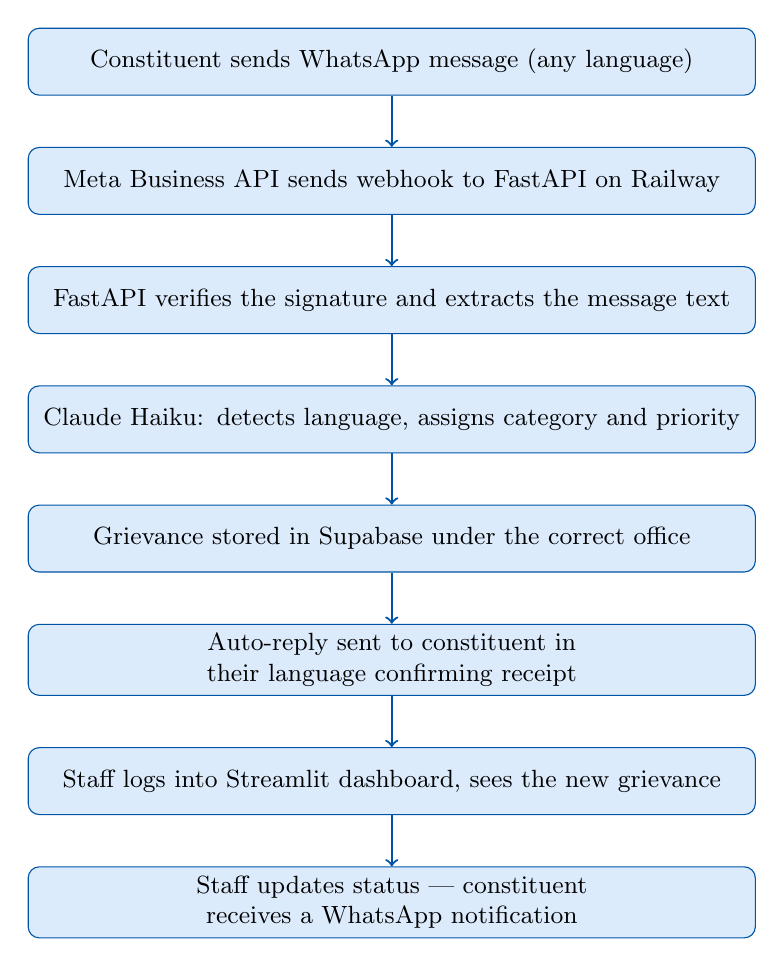
\begin{tikzpicture}[
    node distance=0.65cm,
    box/.style={rectangle, rounded corners=4pt, draw=pollityblue,
                fill=pollitylightblue, text width=9cm, align=center,
                minimum height=0.85cm, font=\small},
    arrow/.style={->, thick, color=pollityblue},
    lbl/.style={font=\scriptsize\itshape, color=darkgray}
]
    \node[box] (n1) {Constituent sends WhatsApp message (any language)};
    \node[box, below=of n1] (n2) {Meta Business API sends webhook to FastAPI on Railway};
    \node[box, below=of n2] (n3) {FastAPI verifies the signature and extracts the message text};
    \node[box, below=of n3] (n4) {Claude Haiku: detects language, assigns category and priority};
    \node[box, below=of n4] (n5) {Grievance stored in Supabase under the correct office};
    \node[box, below=of n5] (n6) {Auto-reply sent to constituent in their language confirming receipt};
    \node[box, below=of n6] (n7) {Staff logs into Streamlit dashboard, sees the new grievance};
    \node[box, below=of n7] (n8) {Staff updates status --- constituent receives a WhatsApp notification};

    \draw[arrow] (n1)--(n2);
    \draw[arrow] (n2)--(n3);
    \draw[arrow] (n3)--(n4);
    \draw[arrow] (n4)--(n5);
    \draw[arrow] (n5)--(n6);
    \draw[arrow] (n6)--(n7);
    \draw[arrow] (n7)--(n8);
\end{tikzpicture}
\end{center}

\vspace{0.5em}

\begin{callout}{pollityblue}{What Is Not in the Flow}
This diagram is the complete MVP. There is no CPGRAMS integration, no fund tracker,
no social media tool, no voice intake, no mobile app. Those are the product roadmap.
This flow --- message in, classified, stored, dashboard, notification out ---
is what needs to work reliably before anything else is built.
\end{callout}

\newpage

% =========================================================================
% SECTION 6: REPOSITORY STRUCTURE
% =========================================================================
\section{Repository Structure}

Two applications. Flat file structure. No infrastructure-as-code.
Everything a new person needs to understand the project is in \texttt{docs/}.

\begin{treebox}
pollity-mvp/
|
+-- backend/                        # FastAPI (Railway)
|   +-- app/
|   |   +-- main.py                 # Entry point, route registration
|   |   +-- config.py               # Settings loaded from environment variables
|   |   +-- database.py             # Supabase client setup
|   |   +-- models.py               # SQLAlchemy ORM models
|   |   +-- schemas.py              # Pydantic request/response schemas
|   |   +-- whatsapp.py             # Webhook handler, HMAC verification, message parser
|   |   +-- classifier.py           # Claude Haiku: language + category + priority
|   |   +-- notifier.py             # Outbound WhatsApp messages to constituents
|   |   +-- grievances.py           # Grievance create, read, update status
|   |   +-- auth.py                 # Supabase JWT verification middleware
|   +-- tests/
|   |   +-- test_webhook.py
|   |   +-- test_classifier.py
|   |   +-- simulate_message.py     # Sends a fake POST to local server for testing
|   +-- requirements.txt
|   +-- Procfile                    # Tells Railway how to start the app
|
+-- dashboard/                      # Streamlit (Streamlit Community Cloud)
|   +-- app.py                      # Entry point
|   +-- pages/
|   |   +-- 1_grievances.py         # Grievance list, filters, status updates
|   |   +-- 2_analytics.py          # Category breakdown, volume chart
|   |   +-- 3_settings.py           # Office profile
|   +-- components/
|   |   +-- auth.py                 # Login form + Supabase Auth integration
|   |   +-- grievance_table.py      # Reusable grievance list
|   +-- requirements.txt
|
+-- docs/
|   +-- architecture.md             # How the system works, in plain English
|   +-- setup.md                    # Running the project locally from zero
|   +-- whatsapp-setup.md           # Meta Business API step-by-step guide
|   +-- data-model.md               # What each table and column stores
|   +-- user-guide-english.md       # Guide for rep office staff
|   +-- user-guide-hindi.md         # Hindi version
|
+-- scripts/
|   +-- seed_data.py                # Insert test offices and grievances
|   +-- check_rls.py                # Verify RLS blocks cross-office queries
|
+-- .github/
|   +-- workflows/
|       +-- ci.yml                  # Run tests on every pull request
|
+-- .env.example
+-- .gitignore
+-- README.md
\end{treebox}

\newpage

% =========================================================================
% SECTION 7: THE HARDEST PARTS
% =========================================================================
\section{The Hardest Parts}

These are the specific places where first-time builders most commonly
get stuck, and why time must be budgeted for them explicitly.

\subsection{Meta WhatsApp Business API Verification (SNVC Week 1)}

Apply on Day 1. The process requires a registered business entity,
a Facebook Business Manager account, a verified phone number, and a
live privacy policy URL. Approval takes 5--14 business days.
If the application is not submitted in Week 1, the webhook cannot be
tested until Week 3 or 4, which compresses the entire build timeline.

\subsection{Webhook Verification and Parsing (SNVC Week 4)}

Meta's webhook system has two parts that must both work before any
messages arrive. First, Meta sends a \texttt{GET} request with a
challenge token --- the server must echo it back correctly or Meta
will not activate the webhook. Second, every \texttt{POST} from Meta
includes an HMAC-SHA256 signature that must be verified. These are
standard patterns but they are new, and they must both work before
a single real message can be processed.

\subsection{Supabase Row Level Security (Phase 2, Weeks 1--2)}

RLS is what ensures that one representative office cannot read another's
grievance data. It is enforced at the database level, not the application
level, which makes it the right approach --- but the syntax and the way
Supabase passes JWT claims to the database session are non-trivial to
set up correctly for the first time. The \texttt{check\_rls.py}
script exists specifically to test this. Run it before onboarding
any real user.

\subsection{Getting Political Users to Change Their Workflow}

This is not technical. It is harder than any of the above.
Representative offices are high-inertia environments. Staff are busy.
Any new tool that requires learning something new will be ignored
unless the person introducing it has personal credibility with the office.

The most effective demo is not a slide deck. It is sending a live
WhatsApp message and watching the staff member's face when the
auto-reply arrives in 10 seconds. That moment is more persuasive
than any pitch. Build toward that demo as early as possible.

\newpage

% =========================================================================
% SECTION 8: DEFERRED ITEMS
% =========================================================================
\section{What Is Deferred}

\renewcommand{\arraystretch}{1.4}
\begin{tabularx}{\textwidth}{X p{2.5cm} X}
\toprule
\rowcolor{pollitylightblue}
\textbf{Item} & \textbf{When} & \textbf{Why Acceptable} \\
\midrule
Next.js / React frontend        & Post-seed   & Streamlit is functional for 50 in-person onboarded users. Time saved not learning React is better spent getting users. \\
AWS Mumbai (DPDP)               & Post-seed   & DPDP enforcement rules not yet finalised. No regulator pursues a pre-revenue startup with 50 users. Migrate before commercial launch. Document the decision. \\
Redis queue                     & Post-seed   & A Supabase jobs table handles the volume for 50 users without issue. \\
CPGRAMS integration             & Post-seed   & Requires a government MOU taking 12--36 months. Not a technical task. \\
Security audit                  & Post-seed   & OWASP Top 10 self-review plus the RLS test script is sufficient for a closed beta. \\
Fine-tuned NLP models           & After beta  & Need real labelled grievance data first. Claude Haiku is accurate enough for beta. \\
Docker and Terraform            & When hiring & Adds weeks of setup with no user-facing benefit at two-person team size. \\
Company incorporation           & Post-seed   & Incorporate once there is revenue or a term sheet to protect. \\
Vidhayak-Mitra, Vikas-Tracker, Nagrik-Setu & Post-seed & All three agents are post-beta roadmap. Jan-Sunwai only for the MVP. \\
\bottomrule
\end{tabularx}

\newpage

% =========================================================================
% SECTION 9: RISK REGISTER
% =========================================================================
\section{Risk Register}

\renewcommand{\arraystretch}{1.5}
\begin{tabularx}{\textwidth}{X p{1.4cm} p{1.4cm} X}
\toprule
\rowcolor{pollitylightblue}
\textbf{Risk} & \textbf{Prob.} & \textbf{Impact} & \textbf{Mitigation} \\
\midrule
Meta API approval delayed past Week 3 & High & High & Apply Week 1 Day 1. Use Telegram Bot API as a development fallback --- same webhook architecture, instant approval. \\
Webhook integration takes longer than one week & High & Medium & Allocate all of Week 4 to this. It is the hardest single technical task. Find anyone who has built a WhatsApp webhook before and ask them to review the code. \\
SNVC coursework and prototype build conflict & High & Medium & The prototype build is sequenced so each week's technical task is small and independent. Falling behind one week does not collapse the whole plan. \\
RLS misconfigured and leaks data between offices & Medium & Critical & \texttt{check\_rls.py} must run and pass before any real user is onboarded. Not optional. \\
Production error with no visibility & Medium & High & Sentry is set up in SNVC Week 2. Every error generates a notification with a full stack trace. \\
50 beta users not reached in Phase 2 & High & Critical & Start user outreach in SNVC Week 2, not after SNVC ends. Aim for 10 verbal commitments before Phase 2 begins. \\
Streamlit too slow or limited & Low & Medium & At 50 users and simple tables it performs adequately. Test on a mobile browser before any real user sees it. \\
One founder runs out of time or motivation & Medium & Critical & Weekly check-in between Piyush and Joe. Scope is fixed; timeline can slip; the team cannot. \\
\bottomrule
\end{tabularx}

\newpage

% =========================================================================
% SECTION 10: THE UPGRADE PATH
% =========================================================================
\section{The Upgrade Path: What SNVC Prize Money Changes}

If Pollity wins SNVC prize money, the Phase 2 build accelerates.
Here is what changes at different funding levels.

\begin{table}[ht]
\centering
\caption{Phase 2 Build at Different Funding Levels}
\renewcommand{\arraystretch}{1.5}
\begin{tabularx}{\textwidth}{p{2.5cm} X X}
\toprule
\rowcolor{pollitylightblue}
\textbf{Funding} & \textbf{What Stays the Same} & \textbf{What Changes} \\
\midrule
\$0 (bootstrap only) & Everything in this document. Railway + Supabase + Streamlit. Piyush and Joe build it themselves over 20 weeks. & Nothing. The plan is viable as written. \\
\midrule
\$10K--50K (partial SNVC prize) & Core stack unchanged. & Hire one part-time contractor for 4--6 weeks to accelerate Phase 2. Consider migrating dashboard to Next.js. \\
\midrule
\$100K+ (full pre-seed) & Core stack unchanged initially. & Migrate to AWS Mumbai (DPDP compliance). Replace Streamlit with Next.js. Begin hiring first full-stack engineer. Start Vidhayak-Mitra scoping. \\
\midrule
\$300K+ (seed round, post-SNVC validation) & Jan-Sunwai v1 is already in production. & Full engineering team. Next.js frontend. AWS infrastructure. DPDP compliance. Begin all four agents in parallel. \\
\bottomrule
\end{tabularx}
\end{table}

\vspace{1em}

\begin{callout}{okgreen}{The Sequence That Leads to the Seed Round}
\begin{enumerate}[leftmargin=1.5em, itemsep=0.3em]
    \item Complete SNVC with a working prototype demo and a strong final pitch.
    \item Whether or not prize money is won, begin Phase 2 immediately after SNVC.
    \item Build Jan-Sunwai v1 on Railway + Supabase + Streamlit over 20 weeks.
    \item Onboard 50 representative offices. Collect NPS $>$ 40, 1,000+ grievances
          processed, 5 case studies.
    \item Use those numbers to raise a \$300--500K seed round.
    \item With seed capital: AWS Mumbai, Next.js frontend, first engineer, Vidhayak-Mitra.
\end{enumerate}

\vspace{0.4em}
\textbf{The strongest investor signal is not the SNVC prize.
It is two founders who built a working product under \$500, put it
in front of 50 political users, and came back with data showing it works.
SNVC validates the idea. Phase 2 validates the business.}
\end{callout}

\vfill
\begin{center}
    {\color{midgray}\rule{0.5\linewidth}{0.5pt}}\\[0.3cm]
    {\small\itshape Pollity --- Building India's Last Mile of Digital Governance}\\
    {\small pollity.in \quad $\cdot$ \quad hello@pollity.in \quad $\cdot$ \quad \textcopyright\ 2026 Pollity}
\end{center}

\end{document}
